%%%%%%%%%%%%%%%%%%%%%%%%%%%%%%%%%%%%%%%%%%%%%%%%%%%%%%%%%%%%%%%%%%%%
%% I, the copyright holder of this work, release this work into the
%% public domain. This applies worldwide. In some countries this may
%% not be legally possible; if so: I grant anyone the right to use
%% this work for any purpose, without any conditions, unless such
%% conditions are required by law.
%%%%%%%%%%%%%%%%%%%%%%%%%%%%%%%%%%%%%%%%%%%%%%%%%%%%%%%%%%%%%%%%%%%%

\documentclass{beamer}
\usetheme[faculty=law,logoPath=./,logo=fudan_logo_vector.eps]{fibeamer}
\usepackage[utf8]{inputenc}
\usepackage{fontspec}
\setsansfont[Scale=MatchLowercase,Mapping=tex-text]{Calibri}
\setmonofont[Scale=MatchLowercase]{Courier New}  
\usepackage[
  % main=english, %% By using `czech` or `slovak` as the main locale
                %% instead of `english`, you can typeset the
                %% presentation in either Czech or Slovak,
                %% respectively.
    czech, 
    slovak,english, %% The additional keys allow foreign texts to be
]{babel}        %% typeset as follows:
%%
%%   \begin{otherlanguage}{czech}   ... \end{otherlanguage}
%%   \begin{otherlanguage}{slovak}  ... \end{otherlanguage}
%%
%% These macros specify information about the presentation
\title{Crystal-amorphous transition based on graphene nanoribbon knot} %% that will be typeset on the
%% \subtitle{} %% title page.
\author{Yang Zhou}
%% These additional packages are used within the document:
\usepackage{ragged2e}  % `\justifying` text
\usepackage{booktabs}  % Tables
\usepackage{tabularx}
\usepackage{tikz}      % Diagrams
\usetikzlibrary{calc, shapes, backgrounds}
\usepackage{amsmath, amssymb}
\usepackage{url}       % `\url`s
\usepackage{listings}  % Code listings
\usepackage{color}

\frenchspacing
\begin{document}
\uselanguage{english}
\frame{
\maketitle \\
{\color{white} \today}
}


\begin{frame}<beamer>
  \frametitle{Outline} %%\thesection
  \tableofcontents\end{frame}
\section{Introduction}
\begin{frame}{Introduction}

  \begin{enumerate}
    \item Crystal-amorphous transition

    \item Knot exists every where and it’s a connection between 1D and 0D materials

    \item Graphene is suitable for the exploring of CAT base on knot
    \item From first principle and classical MD we explore thermal and electronic properties of graphene knot and found it’s a controllable CAT material under uniaxial  stress.

  \end{enumerate}
  \bigskip
  \justifying
\end{frame}


\section{Structure}
\begin{frame}{Structure}
  \framesubtitle{Graphene knot}%
  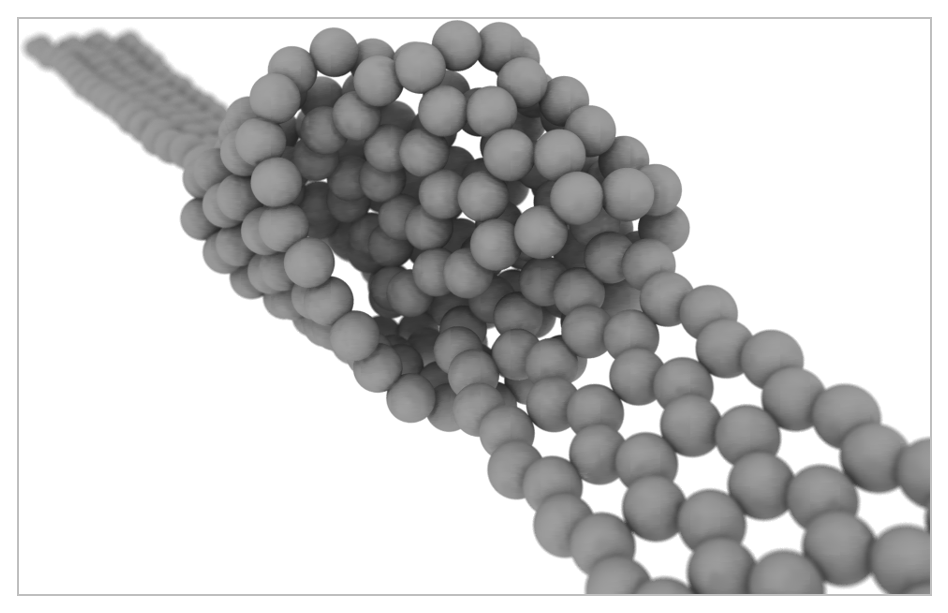
\includegraphics[width=\textwidth]{images/structure}
\end{frame}

\begin{frame}{Break Test}
  \framesubtitle{Multi-time break effect}%
  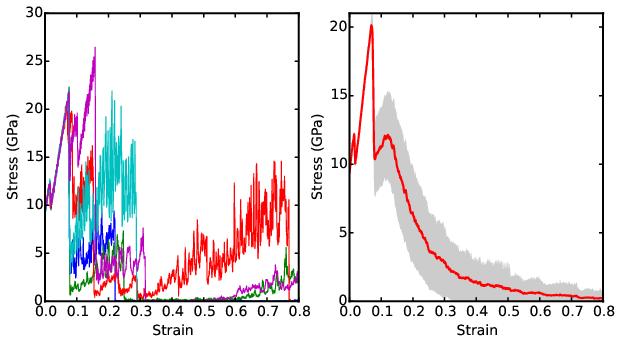
\includegraphics[width=\textwidth]{images/stress}
\end{frame}

\section{Tensile Test}
\begin{frame}{Cycle Test}
  \framesubtitle{Compare to ribbon}%
  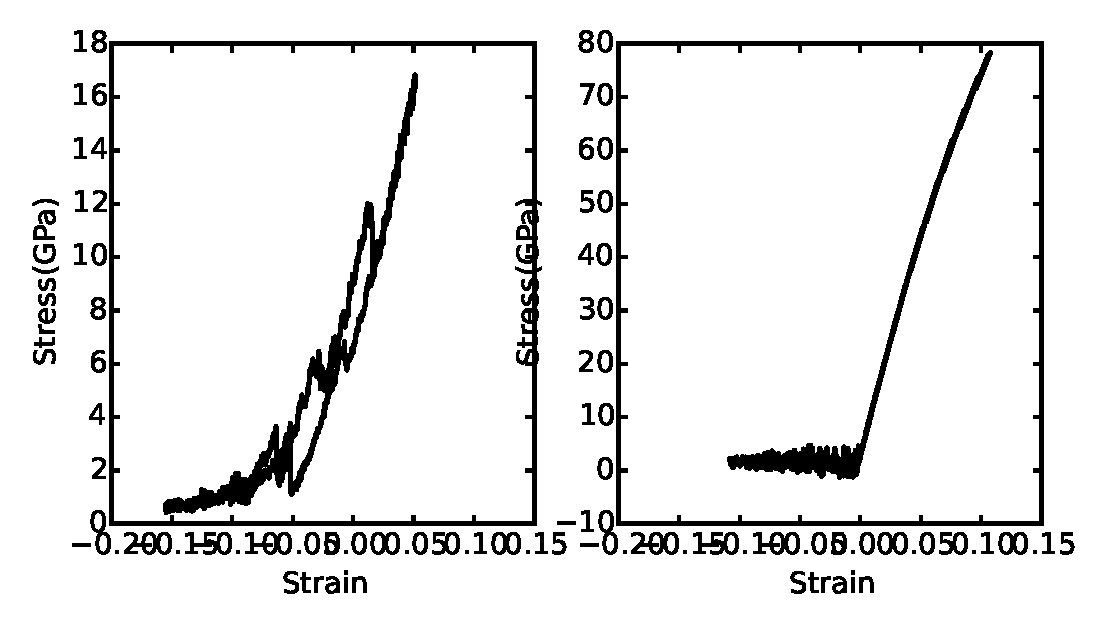
\includegraphics[width=\textwidth]{images/cycle}
\end{frame}


\begin{frame}{Break Test}
  \framesubtitle{Break statics}%
  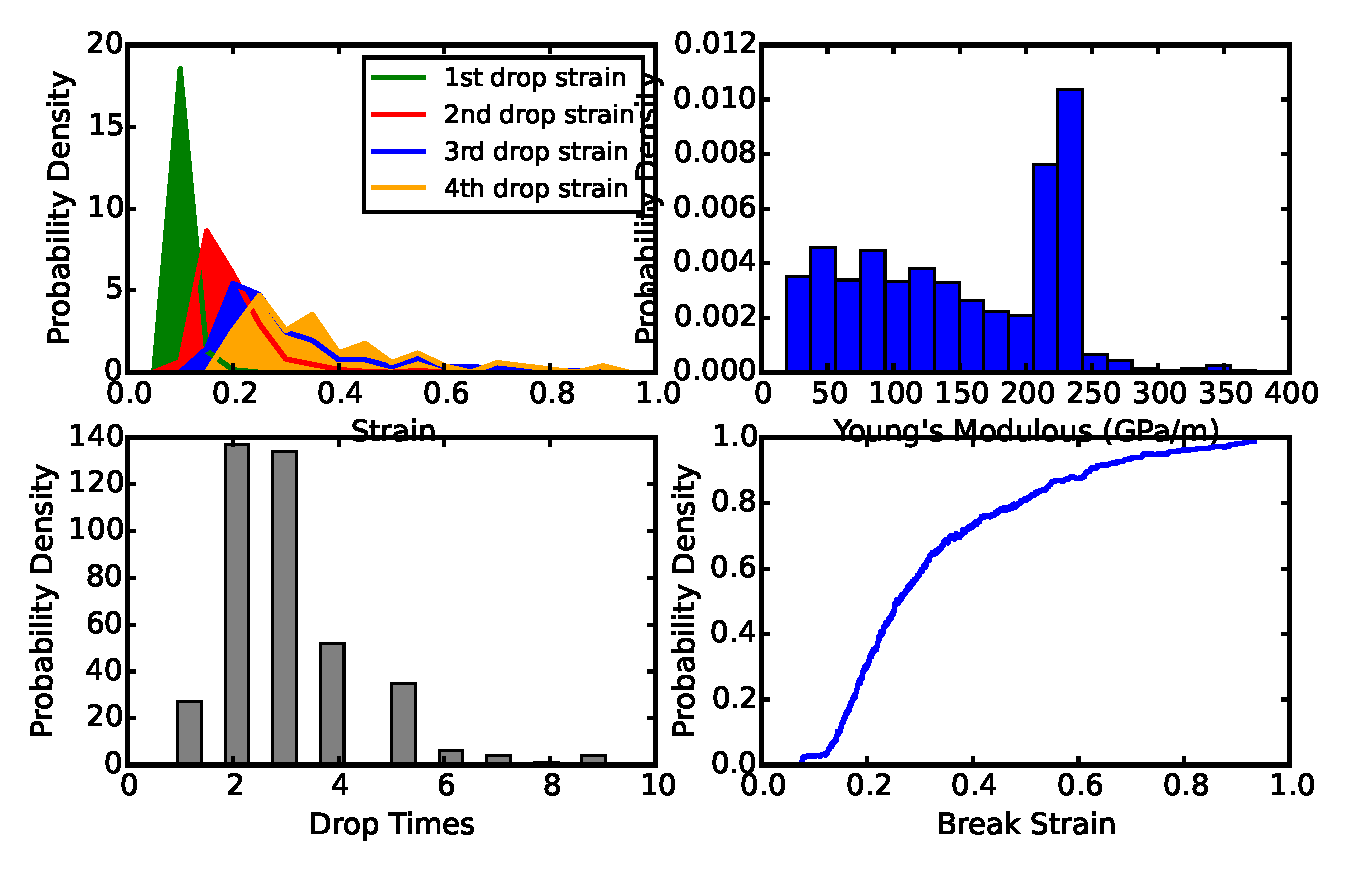
\includegraphics[width=\textwidth]{images/drop}
\end{frame}

\section{Thermal Conductivty}
\begin{frame}{Thermal Conductivty}
  \framesubtitle{Vs. length and strain}%
  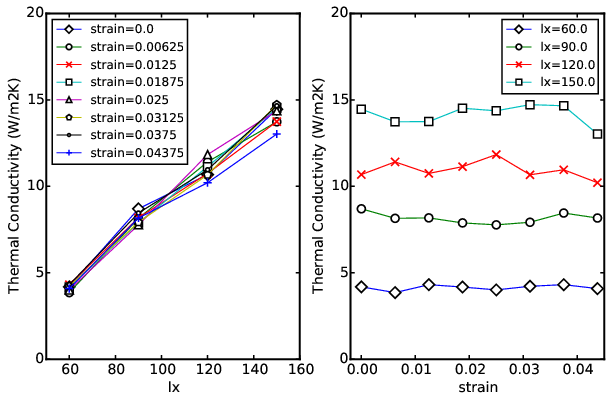
\includegraphics[width=\textwidth]{images/tc_lx}
\end{frame}

\begin{frame}{Thermal Conductivty}
  \framesubtitle{Knot Superlattice}%
  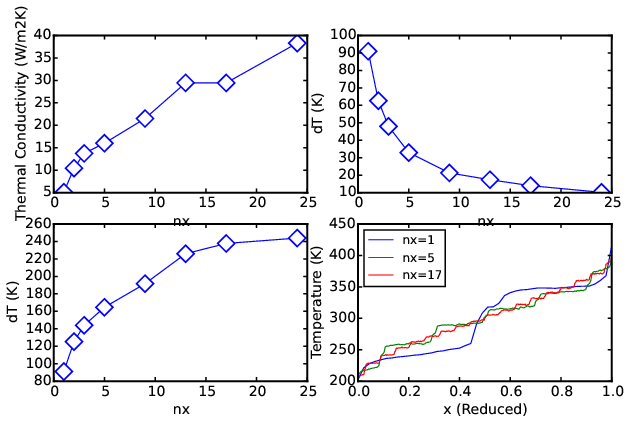
\includegraphics[width=\textwidth]{images/tc_nx}
\end{frame}

\section{Spectrum Analysis}
\begin{frame}{Spectrum Analysis}
  \framesubtitle{Phonon Density of States}%
  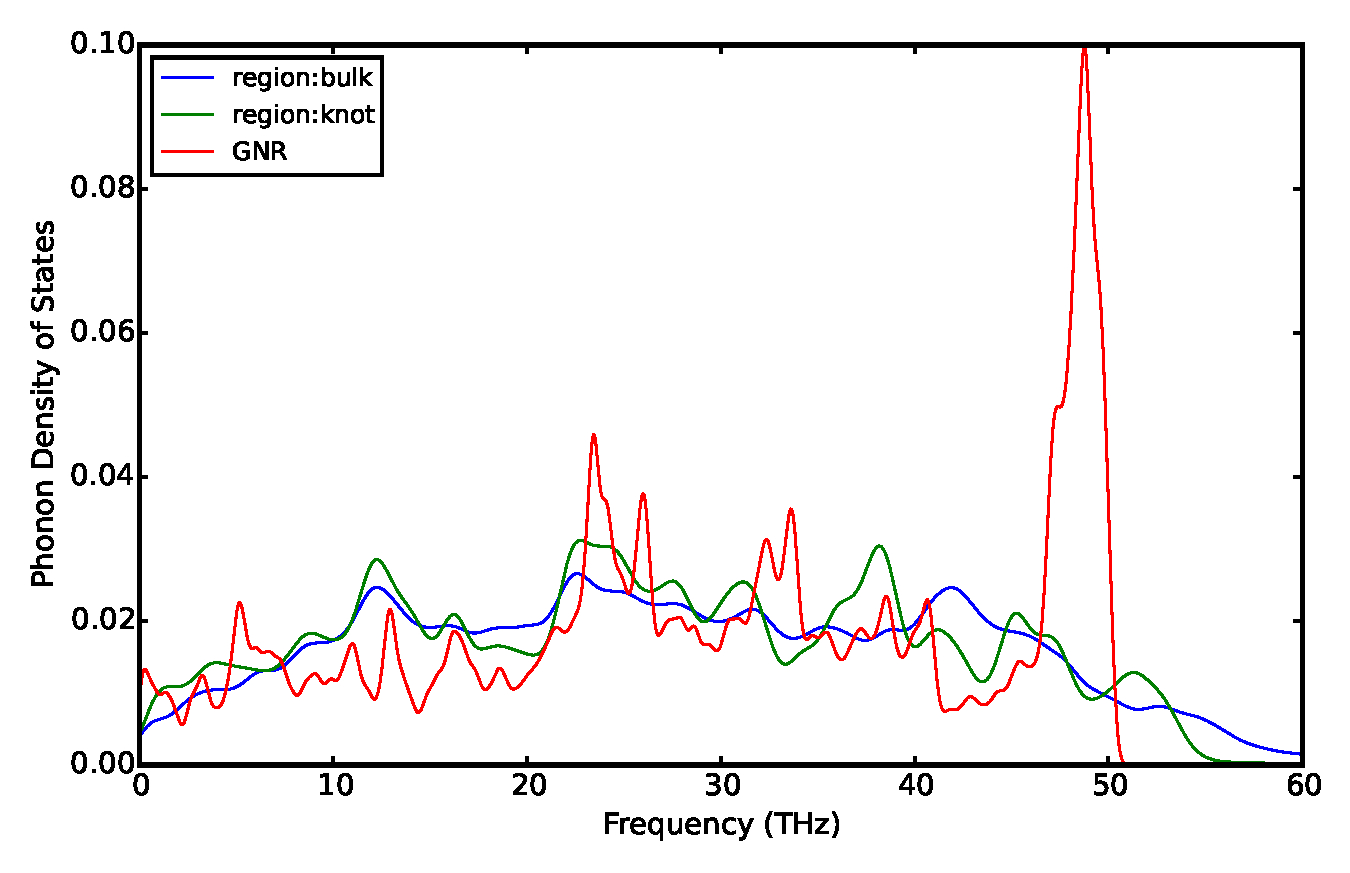
\includegraphics[width=\textwidth]{images/dos}
\end{frame}



\section{Conclusion}
\begin{frame}[label=lists]{Conclusion}

  \begin{enumerate}
    \item layer < 6L
          \begin{itemize}
            \item Large anisotropy(>20\%).
          \end{itemize}
          \begin{itemize}
            \item Reason: Group velosity differrence caused by reconstruction.
          \end{itemize}
    \item layer = 2L
          \begin{itemize}
            \item Most difference due to reconstruction.
          \end{itemize}
          \begin{itemize}
            \item More layer will reduce reconstruction so the anisotropy.
          \end{itemize}
    \item layer < 6L
          \begin{itemize}
            \item TC as low as 1.2 W/mK
          \end{itemize}
          \begin{itemize}
            \item Anisotropy as high as 75\%
          \end{itemize}

          \begin{itemize}
            \item Potential in thermoelectric application
          \end{itemize}
  \end{enumerate}
  \bigskip
  \justifying
\end{frame}


\begin{frame}[label=bibliography]{Bibliography}
  \framesubtitle{\TeX, \LaTeX, and Beamer}
  \begin{thebibliography}{9}
    \bibitem{knuth84}
    Donald~E.~Knuth.
    \emph{The \TeX book}.
    Addison-Wesley, 1984.
    \bibitem{lamport94}
    Leslie~Lamport.
    \emph{\LaTeX : A Document Preparation System}.
    Addison-Wesley, 1986.
    \bibitem{MG94}
    M.~Goossens, F.~Mittelbach, and A.~Samarin.
    \emph{The \LaTeX\ Companion}.
    Addison-Wesley, 1994.
    \bibitem{tantau04}
    Till~Tantau.
    \emph{User's Guide to the Beamer Class Version 3.01}.
    Available at \url{http://latex-beamer.sourceforge.net}.
    \bibitem{MS05}
    A.~Mertz and W.~Slough.
    Edited by B.~Beeton and K.~Berry.
    \emph{Beamer by example} In TUGboat,
    Vol. 26, No. 1., pp. 68-73.
  \end{thebibliography}\end{frame}


\end{document}
